%\documentstyle[epsf,twocolumn]{jarticle}       %LaTeX2e仕様
\documentclass[twocolumn]{ujarticle}     %pLaTeX2e仕様(platex.exeの場合)
%\documentclass[twocolumn]{ujarticle}     %pLaTeX2e仕様(uplatex.exeの場合)
%%%%%%%%%%%%%%%%%%%%%%%%%%%%%%%%%%%%%%%%%%%%%%%%%%%%%%%%%%%%%%
%%
%%  基本バージョン
%%
%%%%%%%%%%%%%%%%%%%%%%%%%%%%%%%%%%%%%%%%%%%%%%%%%%%%%%%%%%%%%%%%
\setlength{\topmargin}{-45pt}
%\setlength{\oddsidemargin}{0cm} 
\setlength{\oddsidemargin}{-7.5mm}
%\setlength{\evensidemargin}{0cm} 
\setlength{\textheight}{24.1cm}
%setlength{\textheight}{25cm} 
\setlength{\textwidth}{17.4cm}
%\setlength{\textwidth}{172mm} 
\setlength{\columnsep}{11mm}

\kanjiskip=.07zw plus.5pt minus.5pt


% 【節が変わるごとに (1.1)(1.2) … (2.1)(2.2) と数式番号をつけるとき】
%\makeatletter
%\renewcommand{\theequation}{%
%\thesection.\arabic{equation}} %\@addtoreset{equation}{section}
%\makeatother

%\renewcommand{\arraystretch}{0.95} 行間の設定

%%%%%%%%%%%%%%%%%%%%%%%%%%%%%%%%%%%%%%%%%%%%%%%%%%%%%%%%
\usepackage[dvipdfmx]{graphicx}   %pLaTeX2e仕様(\documentstyle ->\documentclass)\documentclass[dvipdfmx]{graphicx}
\usepackage[subrefformat=parens]{subcaption}
%%%%%%%%%%%%%%%%%%%%%%%%%%%%%%%%%%%%%%%%%%%%%%%%%%%%%%%%

\begin{document}
	
	\twocolumn[
	\noindent
	
	\hspace{1em}
	\today
	\hfill
	\ \ 細川 岳大
	
	\vspace{2mm}
	
	\hrule
	
	\begin{center}
		{\Large \bf 進捗報告}
	\end{center}
	\hrule
	\vspace{3mm}
	]

% ‚ここから 文章 Start!
\section{今週やったこと}
 GAを用いたDataAugmentaion

\section{実験}
前回に引き続きGAを用いたDataAugmentationの実験を行った.
\begin{table}[h]
	\centering
	\caption{学習パラメータ\label{tb:param}}
	\scalebox{0.9}{
		\begin{tabular}{|c||c|} \hline
			optimizer&Adam\\ \hline
			learning rate&0.001\\ \hline
			loss function&categorical\_crossentropy\\ \hline
			batch size&128\\ \hline
		\end{tabular}
	}
\end{table}
表\ref{tb:param}に学習パラメータを示す.
事前学習ではepoch数300,train\_dataを各ラベル5000枚の計50000枚使用し,GAで学習する際はepoch数100,train\_dataは各ラベル200枚のオリジナルとそれらすべてをDataAugmentaionしたものとを合わせ計4000枚とし,test\_dataは共に10000枚とした.
\subsection{実験1}
 前回行った実験に関して30世代まで実験を回した.表\ref{tb:param1}に設定を示す.
\begin{table}[h]
	\centering
	\caption{実験1\label{tb:param1}}
	\scalebox{0.9}{
		\begin{tabular}{|c|c||} \hline
			個体数&10\\ \hline
			交叉率&0.5\\ \hline
			突然変異率&0.2\\ \hline
		\end{tabular}
	}
\end{table}

%図\ref{fig:exp1}に結果を示す

\begin{figure}[t]
	\centering
	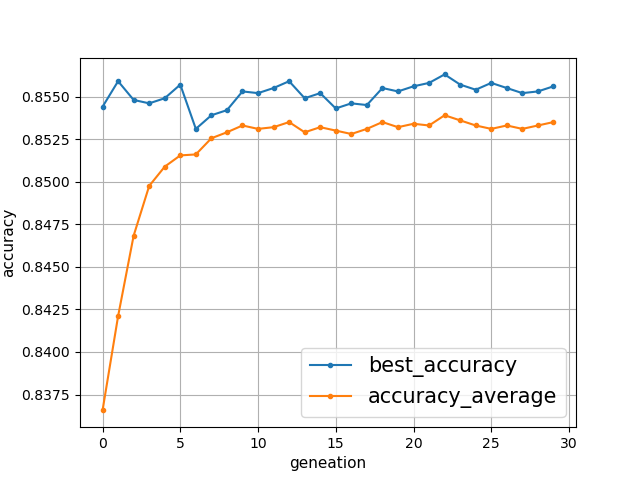
\includegraphics[width=\linewidth]{figure1.png}
	\caption{実験1\label{fig:exp1}}
\end{figure}

accuracyの平均値が最良値に近づいており,遺伝子がそろってきていることが分かる.
しかし,交叉に用いる上位個体が20世代から30世代まで変わらなかった.理由として1世代の個体数が
少ないためすぐに収束したと考えられる.また,学習済みモデルから学習させたことでもとの学習データと大幅に違う画像を生成する個体がすぐにはじかれてしまったのではないかと考えた.


\subsection{実験2}
実験1を踏まえ,個体数,突然変異率を増やし,学習済みモデルを用いずに学習を行った.

表\ref{tb:param2}に設定を示す.
\begin{table}[h]
	\centering
	\caption{実験2\label{tb:param2}}
	\scalebox{0.9}{
		\begin{tabular}{|c|c||} \hline
			個体数&20\\ \hline
			交叉率&0.5\\ \hline
			突然変異率&0.4\\ \hline
		\end{tabular}
	}
\end{table}

図\ref{fig:exp2}に結果を示す

\begin{figure}[b]
	\centering
	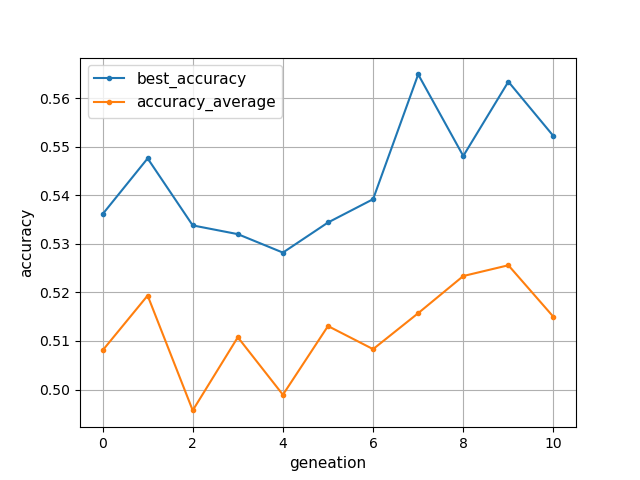
\includegraphics[]{figure2.png}
	\caption{実験2\label{fig:exp2}}
\end{figure}

まだ世代数が少ないため良い個体が出現しなかっただけかもしれないが,全体的に精度自体が良くなく,
ある程度学習されたモデルからはじめなければならないか,あるいは水増しされたミニデータ自体の個数を増やすかしなければ,
学習済みモデルを用いたものに近しい精度が得られないと思う.

\section{今後の課題}
\ 精度を上げるには個体数,ミニデータ数,世代数どれに関しても上げていかなければならない.
または識別クラス数を減らしてより簡単なタスクで行ってみるなど.


\end{document}


